\section{System Implementation} 
hue hue hue

\subsection{Gesture Recognition}
\subsubsection{Preprocessing}
Once the acceleration and rotation data is sent from the device to the computer,
 the values are smoothed with an average of the 20 previous values in order to avoid and reduce the effect of noise on the sensors.
 This phase is called preprocessing of the data. 
 This allowed us to have more precise information, as can be deducted from the images  \ref{fig:figure2} and \ref{fig:figure3}

\begin{figure}[!h]
\centering
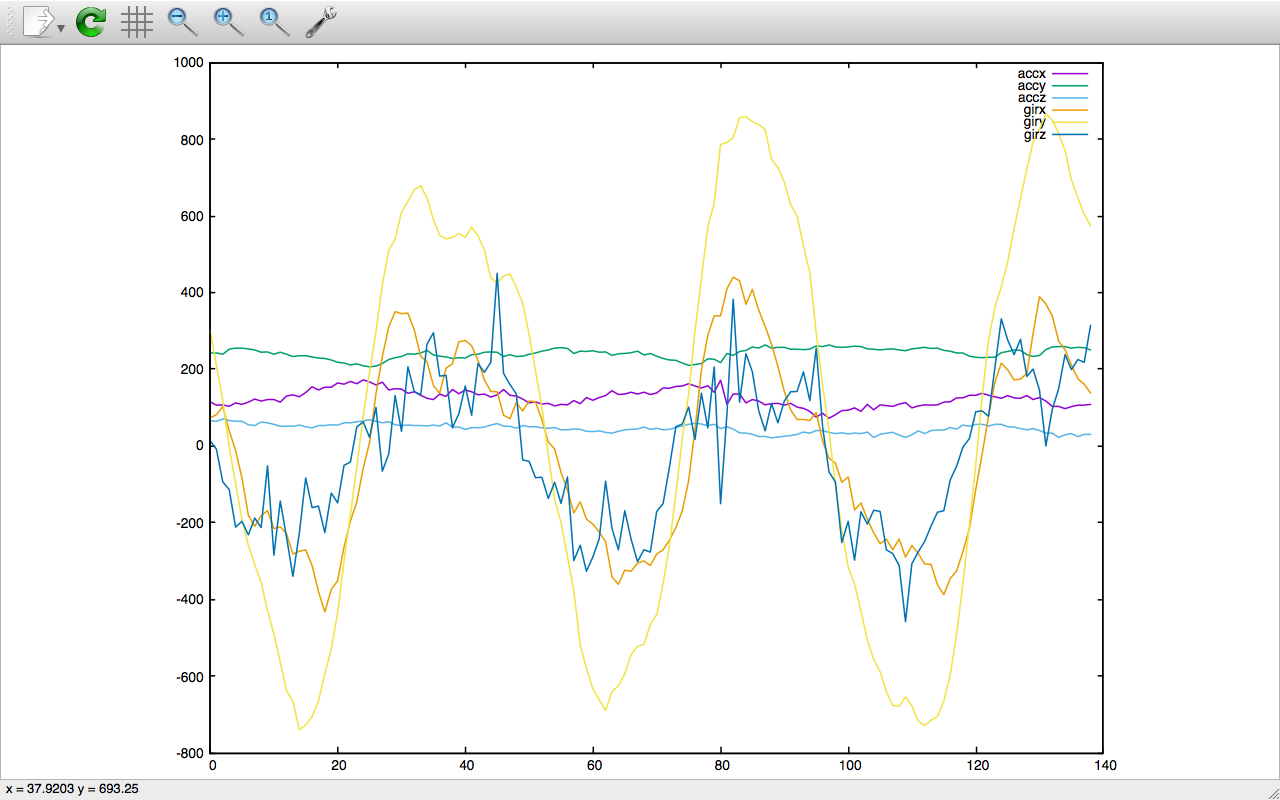
\includegraphics[width=0.9\columnwidth]{img/raw}
\caption{Data from the device before preprocessing.}
\label{fig:figure2}
\end{figure}

\begin{figure}[!h]
\centering
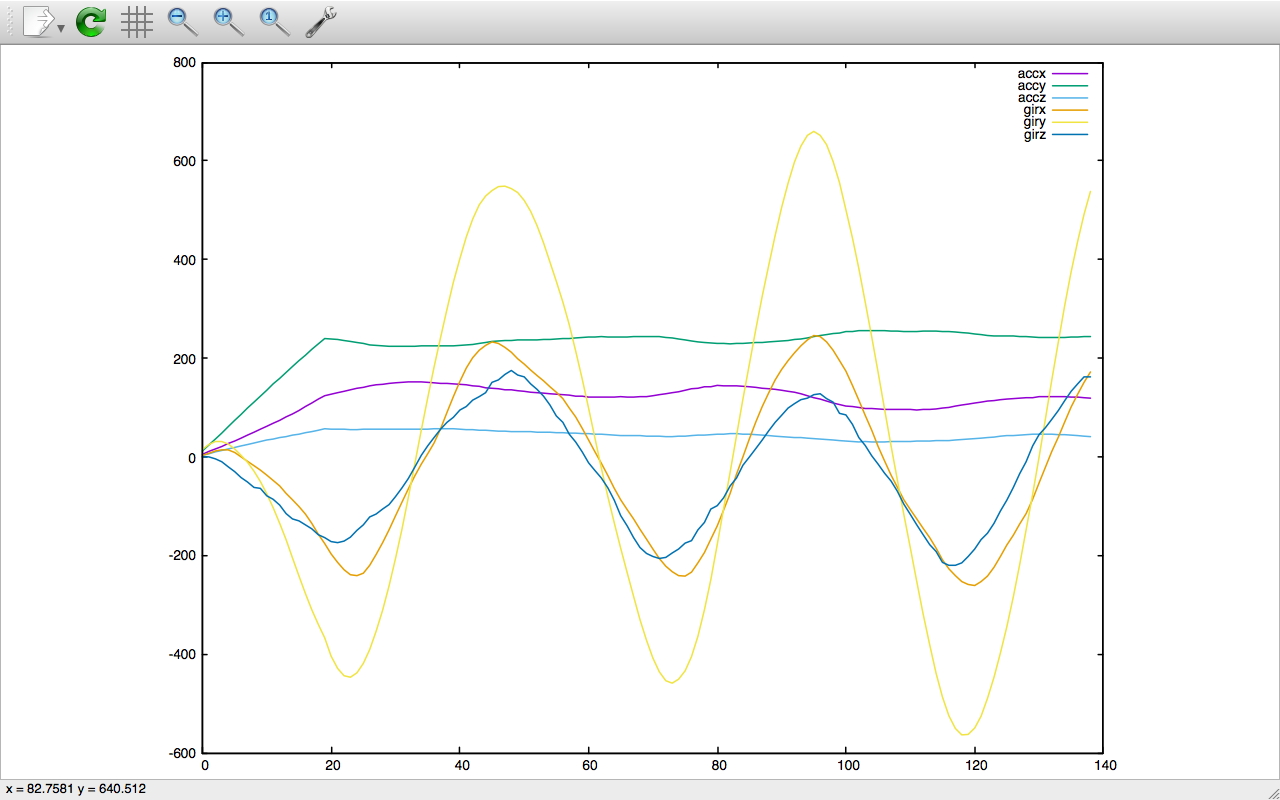
\includegraphics[width=0.9\columnwidth]{img/20}
\caption{Data from the device after preprocessing.}
\label{fig:figure3}
\end{figure}

\subsubsection{Evaluation}
For the actual processing and gesture recognition, we organized known gestures in a very large training set, each individual gesture stored as a list of 50 * 6 values plus an identifier. 
The training data set in the final version of the project reached more than 500 entries in total.
We use Weka 3.6 to evaluate newly received data using a BayesNet classifier and comparing it to the training set. 
This resulted as the most accurate classifier for our model, giving up to 100\% accuracy when testing it.
The evaluation of the gesture is performed every 10 * 6 new values received.

\subsection{Technical challenges}